 


\section{Q1}
\label{part1}
\begin{enumerate}


\item Choose 100 URIs from A1

\item Generate WARC files of those URIs using:
- wget
- WARCreate
- Heritrix (standalone or via WAIL)
- webrecorder.io

\item Describe the resulting WARC files: quantitatively compare and contrast the results of the WARC files of the same URI as generated by different tools 
- choose interesting examples

 \item Demonstrate playback of 2-3 WARCs in the (Wayback Machine (via WAIL or stand-alone) or pywb) and (webrecorder.io)
- https://github.com/iipc/openwayback 
- https://github.com/ikreymer/pywb 


\end{enumerate}

\subsection{Description}


\begin{enumerate}

\item The WARC files contain all the request headers, response headers and the html to render the recorded webpage.

\item The WARC file size generated by wget is the least amongst all the tools.

\item For few URLs, WARCreate did not generate WARC file despite of trying multiple times.

\item I replayed different WARC files using webrecorder.io and included the screenshots in this report

\item I was having problem with pywb and hence was not able to replay the WARC files on it.


\end{enumerate}

\newpage


\subsubsection{Replay of Different WARC files on webrecorder.io}
\begin{figure}[ht]    
    \begin{center}
        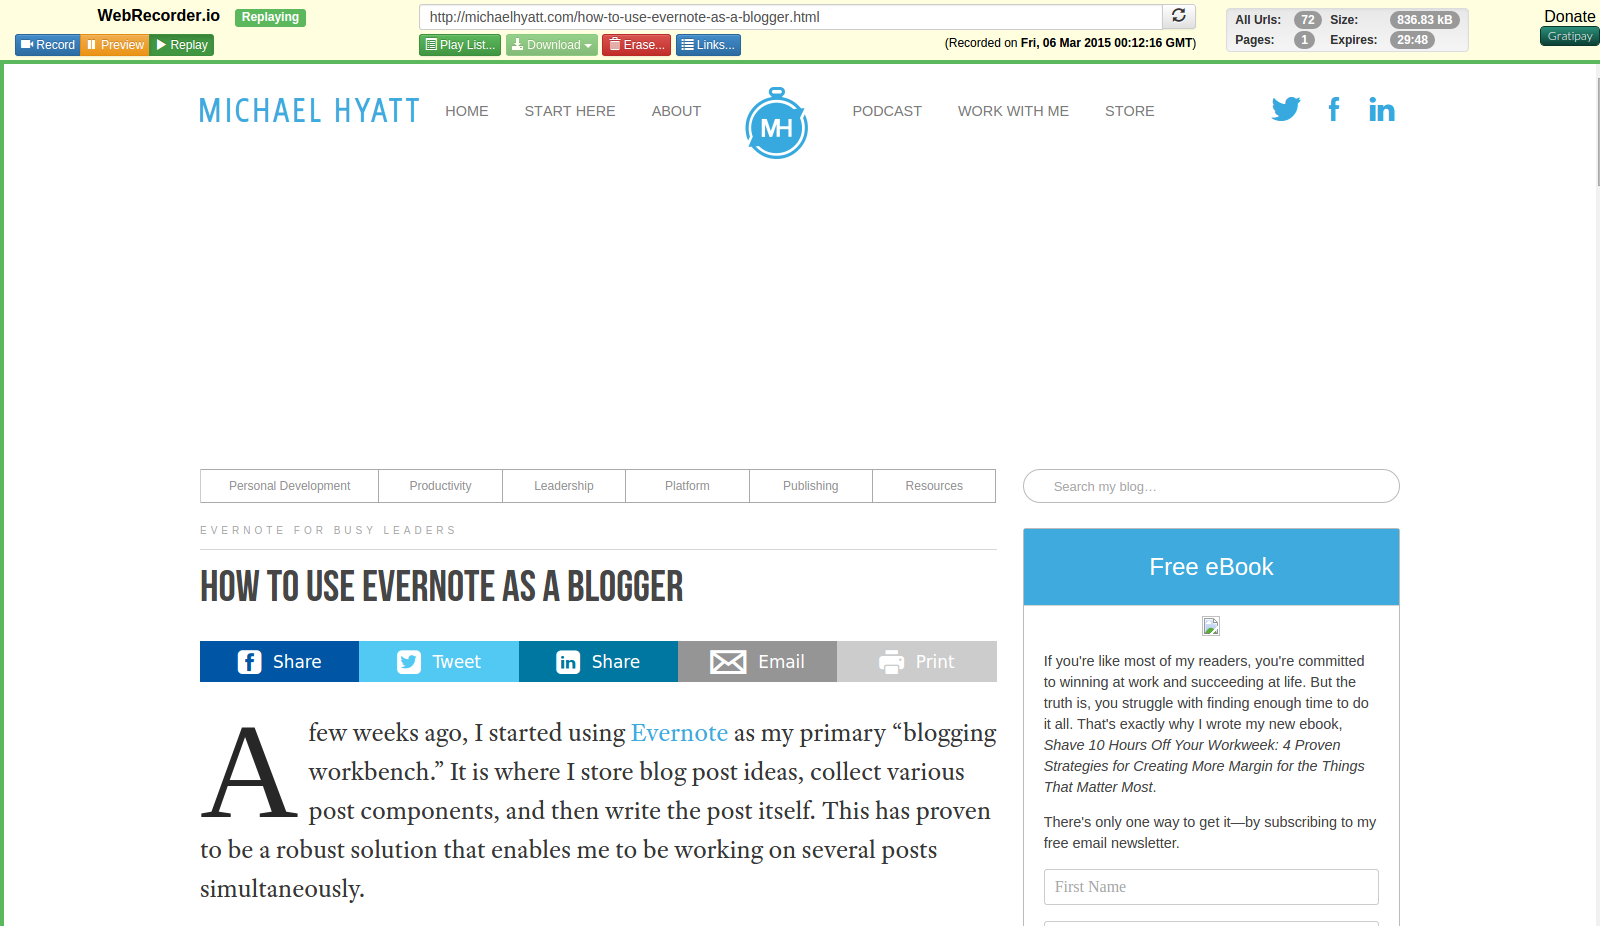
\includegraphics[width=\paperwidth]{warc-replay-1.png}
        \caption{}        
    \end{center}
\end{figure}

\begin{figure}[ht]    
    \begin{center}
        
\includegraphics[width=\paperwidth]{warc-replay-2.png}
        \caption{}
    \end{center}
\end{figure}

\begin{figure}[ht]    
    \begin{center}
        
\includegraphics[width=\paperwidth]{warc-replay-3.png}
        \caption{}
    \end{center}
\end{figure}






